\chapter{Overview of Virtual Memory}
\label{chapter:vm_overview}

In this chapter I will present the most essential information about Virtual Memory subsystem.
We will see how it helps with memory management, what we expect from it and what are the mechanisms that build the virtual memory subsystem.
The implementation details are left for the next chapters (\ref{chapter:details} and \ref{chapter:mimiker}).

\section{Memory in the Operating System}

There are several types of memory used in computer systems.
Different types of memory have different characteristics, the most important of which is access time.
From the user's point of view, it would be ideal to have equal, fast access to all available memory.
On the other hand, it is impossible because there are some limitations:
\begin{itemize}
  \item Fast memory is more expensive to manufacture.
  \item To achieve fast access times, the memory must be physically close to the CPU.
  \item The size of fast memory is limited by its location on the chip.
\end{itemize}

With this in mind, we can place different types of storage in a hierarchy.
At the top we have fast memory types, but with limited size.
As we go down, the memory becomes larger, cheaper, and slower.
(The hierarchy can be seen on the figure \ref{fig:memory_hierarchy}).

In computer systems, each level of the storage hierarchy is used to cache data from levels below it.
(For example, data stored on disk is fetched into RAM to perform operations on it.)
The result is that data that is currently in use is stored in faster memory,
while data that is not currently needed is stored in larger memory.

\begin{figure}[h]
  \centering
  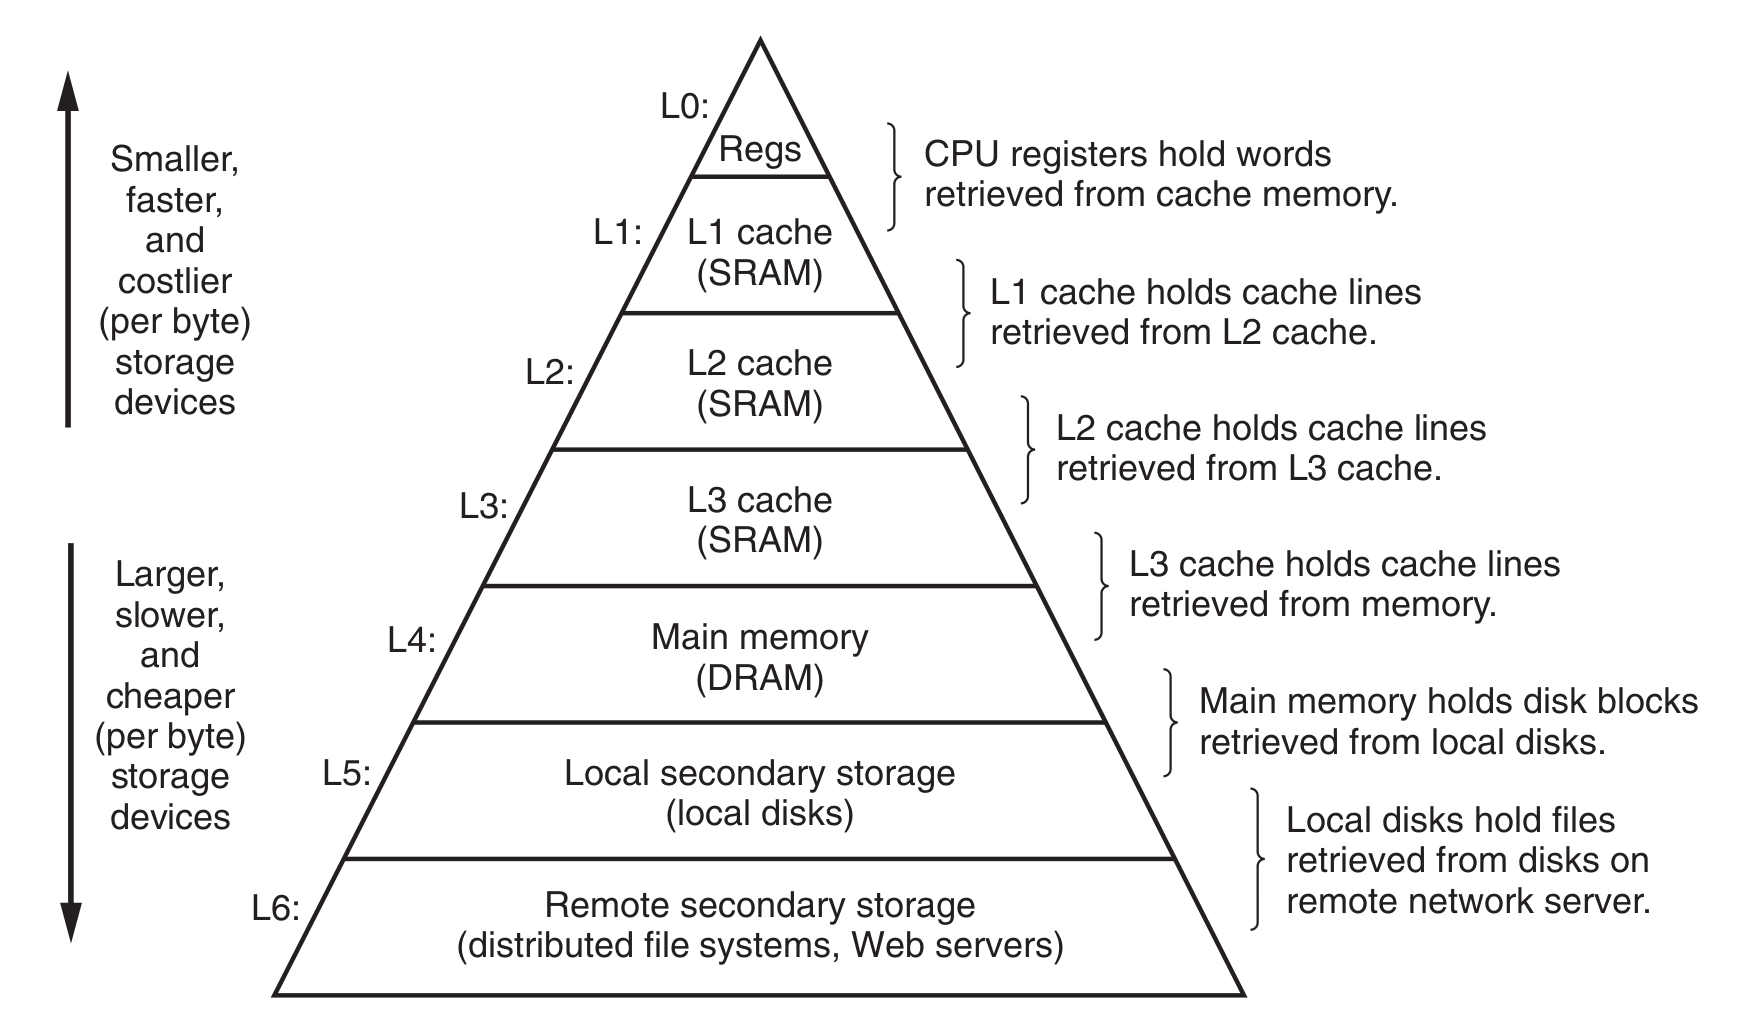
\includegraphics[width=\textwidth]{memory-hierarchy.png}
  \caption{Memory hierarchy in the operating system \cite{csapp}}
  \label{fig:memory_hierarchy}
\end{figure}

\subsection{Problems of physical memory management}

In complex systems there is a need to run multiple programs at the same time.
If~all of them were using memory directly through physical addresses, there would be problems with safety and performance.

The primary challenge with physical memory is that each process must occupy a different region of memory.
They have to use only the addresses that are inside their part of memory and shouldn't be able to modify other processes memory.
This applies to all user processes as well as the OS kernel, which memory shouldn't be even seen by user processes for safety reasons.

To address these issues, programs must be written in such a way that they can be placed at any address in memory.
There should also be hardware mechanisms designed to validate all memory accesses, ensuring that they do not violate the process's access rights.
Although there is one issue that is really hard to solve -- the memory fragmentation.
Since programs use contiguous chunks of memory, there must be a large enough contiguous memory region available for each new program loaded.
Additionally, smaller programs that consume less memory will leave small chunks of unoccupied memory after they exit.
These fragments form gaps that cannot be merged into to be used by a larger program because they are not adjacent.

There are few limitations regarding the size and number of programs running in the OS.
When the program is run, all of its memory must be in RAM occupying a contiguous region.
This means that programs cannot use more memory than is available in the system, even if they are only using a small portion of it at any given time.
Also the number of processes running concurrently is limited, because they all have some amount of memory allocated.
At some point there would be not enough free space to load a new program.

To address the last issue, some running programs may be suspended, and moved to other storage (e.g. to disk) to make room for new program.
Although such solution is inefficient, because whole memory of suspended processes must be copied to different storage (usually with higher latency).

\subsection{Virtual memory}

Virtual memory is a concept invented in 1960s by researchers working on the Atlas computer \cite{denning}.
It was designed to overcome the problems with manually maintaining the memory use of the programs.
By providing a abstraction over physical memory it enables new actions that were not possible earlier.
In this section there is an overview of main concepts used nowadays in virtual memory systems.

\subsubsection{Separate address spaces}

In systems with virtual memory all running processes have their own address space.
{\it Address space} is a set of addresses available and private to a single process.
These addresses are not real, and are not used to access main memory directly.
To distinguish the real and artificial addresses we use two different names for them: {\it virtual addresses} -- for addresses used by the process, and
{\it physical addresses} -- used to describe physical memory.
During a memory access performed by the process, the virtual address specified by the process must be translated to the physical address,
using dedicated kernel mechanism.

The use of separate address spaces makes it easier to isolate different processes.
It is not possible for a process to express the location in the address space of another process in terms of addresses known to itself.
Even if two processes use addresses that are identical because they have the same numerical value, the actual memory access is usually made
to different locations in main memory, due to address translation.

\subsubsection{Paging}

{\it Memory paging} is the technique that helps to manage memory effectively.
It divides both physical memory and virtual address space into equally sized chunks, typically 4 kilobytes large.
When we talk about physical memory, these chunks are called {\it frames}, and in virtual memory they are called {\it pages}.
Later, the virtual pages are associated with physical frames during the address translation using a page table which are both described in more details in \ref{section:address_translation}.

Each page is controlled individually and can either be in main memory or in secondary storage.
Also the location of physical frame used to store contents of memory is not relevant, because of address translation.
That means, that programs can be either partially loaded (when they operate only on few pages) or scattered across whole memory.
The ability to load only part of process memory to RAM makes it possible to run programs that use more memory than the size of RAM.

In addition to that, programs will usually start faster, because only few page has to be allocated to run the program at the beginning.
New pages, with new data or more fragments of program code, will be loaded on demand.

From safety perspective, processes has more control over attributes of allocated memory.
Each page may have different access rights specified, according to their purpose (e.g. process usually shouldn't be able to modify its instructions).
Additionally, kernel can use other page attributes to decide how it is saved or fetched form the backing storage.

\subsubsection{Memory sharing}

In system that uses virtual memory it is possible to precisely define which fragments of process memory are shared with other processes.
Such memory regions are mapped, during address translation, to the same physical pages.
Shared memory can be used to share common data, like program code or shared system libraries.
The other application is to use shared memory as a method of inter-process communication.

\section{Virtual Memory mechanisms}

There are three main mechanisms that work almost all the time when the system is running.
They provide the implementation of the concepts shown in the previous section, and work almost unnoticed by user processes.
Here we will look at the details of address translation, memory swapping, and memory fault handling.

\subsection{Memory swapping}

% DEFINED: swapped out, page daemon, backing storage, wired/pinned pages

The amount of physical memory available to the processes and kernel is limited.
Usually it is too small to store all data of all processes at the same time and sometimes even single process
may want to allocate more memory than it is physically available.
But in fact, programs don't use all of their memory at once, hence it is possible to provide different parts of memory at different times.

The illusion that all memory of the process is available in the main memory is maintained by constantly swapping unused memory pages
with the ones that are required by the process to keep running.
When a process is trying to access memory that isn't currently in RAM memory, then the page fault is triggered.
In this situation the OS kernel is responsible for finding proper page and making it available for the process.
To do this, it sometimes has to free another unused page to make a room for a new one.

To analyze the behaviour of the process in terms of using memory we define a {\it working set} to be the set of pages currently used by the process.
The working set is constantly changing over the time, but some programs have well defined stages that use different fragments of their memory.
(For example, compilers use different code and operate on different parts of the input data for different stages of compilation.)
Programmers can take advantage of this by designing programs so that the entire working set fits into main memory.
The running process will then cause as few page faults as possible, because most of the data used is already in memory.
However, if the process is poorly designed and the working set is larger than the amount of memory available to the process,
it may experience performance problems due to a high page fault rate, because used memory is constantly being swapped.
Such situation is called {\it trashing}.

%* Memory is usually not sufficient to hold all process memory \\
%  - Some other processes are using it too \\
%  - program may require large amount of memory \\
%  - but not all memory is used at once \\
%  - working set - set of pages currently used by the process (e.g. code and data used in single stage of compiler) \\
%  - when whole working set fits into memory process cause not many page faults \\
%  - When working set is too big, process will cause much more page faults. Process is trashing. \\

\subsubsection{Swapping pages}

When system is running out of space it starts to move some pages from main memory to secondary storage.
The process of moving page out of main memory is called {\it swapping out}.
To determine which pages should be swapped out kernel uses a {\it page replacement algorithm}.
The process that is walking through all pages and selecting ones to remove is typically called {\it page daemon}.

When a page is selected to be removed from memory, its contents must be stored somewhere so that the page can be recovered when it is needed again.
The place where page can be saved is called {\it backing storage} or {\it backing store}.
There are two most common backing stores: a swap partition and a file system.

Sometimes, to reduce the number of actions needed to swap out a page, kernel maintains information about modified pages.
Pages that were not modified and are already in the backing storage don't have to be copied there.
They can just be removed from main memory without losing any information about them.

\subsubsection{Page replacement algorithms}

Copying memory is expensive, especially from disks, which typically have high latency.
Therefore system is performing better when it does as little copying as possible.
There are many page replacement algorithms that are trying to achieve smallest possible number of page swaps.
All algorithms try to predict what pages won't be used in the near future, because those are the best candidates to swap out.

\begin{description}[style=nextline]
  \item[Optimal]
    The best possible strategy would be to check which page will not be used or will be used but after some time.
    Such algorithm is impossible because it requires to know future memory accesses.
    Even if that could be determined for some processes it is impossible in general.

  \item[FIFO]
    First in First out algorithm assumes, that the page that was used earlier will not be used for some time.
    In result pages are removed from the memory in the same order they were inserted.

  \item[LRU]
    Least Recently Used algorithm tries to find pages that were unused for some time.
    Kernel maintains the information about which pages were used in the past.
    Pages that were used are more likely to be used again.

  \item[Second chance]
    This algorithm implements a FIFO queue but with additional bit indicating if page was recently used.
    When some page is popped from the queue and wasn't referenced then it is freed.
    Otherwise, when its reference bit was set, it is inserted again on the page queue, with referenced bit unset.

\end{description}

%* Page replacement policies \\
%  - FIFO \\
%  - Optimal \\
%    - algorithm that requires knowledge of future access operations \\
%  - LRU \\
%    - hard to approximate in hardware \\
%    - few simplified algorithms (referenced bit, simple timer) \\
%  - Second chance page replacement alg \\
%    - FIFO on circular buffer with referenced bit \\
%    - When page is referenced, its bit is cleared and it is given a second chance \\
%    - if page is actually being used the referenced bit will be set before it will be considered again \\
%
\subsubsection{Locking pages in memory}

Sometimes there is a need to lock some pages in memory because they hold critical data or are used.
There are two categories of locked pages:

\begin{itemize}
  \item {\bf wired pages} -- such pages can't be swapped at all. Usually huge part of kernel is protected from being swapped.
    It contains critical code needed for some operations made by the kernel.
    Wired pages don't cause page fault, because they are always in the memory.

  \item {\bf pinned pages} -- temporarily wired pages of processes.
    For example, pages are sometimes pinned when a process is doing an I/O operation and its results are saved on that page.
\end{itemize}

%* Locking page in memory
%  - wired pages - in memory all the time - kernel pages
%  - pinned pages - temporarily not swappable - buffers for I/O operations done by process

\subsection{Address translation}
\label{section:address_translation}

To use virtual addresses, they must be translated into physical addresses, because main memory is addressed by physical addresses.
The translation is done by hardware unit called {\it Memory Management Unit (MMU)}, using special structures prepared by the kernel.

Every virtual address used must be mapped to a physical address, and the kernel keeps track of these mappings.
It would be impossible to describe such mappings for every single memory cell, and that is another area where memory paging helps.
Memory is divided into chunks of constant size, typically 4 kilobytes.

During address translation, the MMU splits each address into two parts: {\it virtual page number (VPN)} and {\it page offset} (figure~\ref{fig:address}).
The page number is used to find the {\it physical frame number (PFN)} in the {\it page table} -- structure managed by the kernel.
Next, the frame number and page offset are concatenated to create a physical address, which is used to reference a single memory cell.

More detailed description of address translation can be found in 7.4 of \cite{silberschatz}.

\begin{figure}
  \centering
  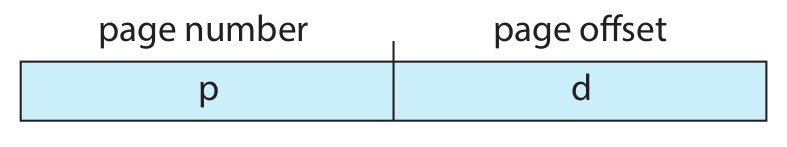
\includegraphics[width=0.5\textwidth]{address.png}
  \caption{Division of an address during address translation \cite{silberschatz}}
  \label{fig:address}
\end{figure}

\subsubsection{Page table entry details}

% DEFINED: page table entry, pte

{\it Page table entries (PTE)} are the elements of page table that describe a single mapping from virtual to physical address.
They must include all the information needed to determine physical frame location and some additional info used to check if memory access made by process is valid.
Page table entry usually contains:

\begin{itemize}
  \item {\bf Physical or virtual address}
    -- needed to identify the mapping.
    Usually only one of these addresses is stored because the second one is used to index the table.

  \item {\bf Access protection}
    -- information about operations that are allowed to perform on given memory.

  \item {\bf Valid bit}
    -- tells if the mapping is valid.
    Only valid mappings can be used by MMU to perform address translation.

  \item {\bf Address space identifier}
    -- (ASID) identifies the process which is using that page.
    Only pages with ASID matchin current process might be used to address translation.

  \item {\bf Dirty bit}
    -- determines if page was modified by the process.
    This information is used when page must be swapped out to avoid unnecessary writes to backing storage.

  \item {\bf Accessed bit}
    -- tells if any access (either read or write) was made to that page.
    This information used when searching for a page to swap out.
\end{itemize}

The set of attributes described in PTE varies between different architectures.
In Mimiker, each architecture has its own header describing the layout of the page table entries:
\href{https://github.com/cahirwpz/mimiker/blob/master/include/aarch64/pte.h}{\tt include/aarch64/pte.h},
\href{https://github.com/cahirwpz/mimiker/blob/master/include/mips/tlb.h}{\tt include/mips/tlb.h},
\href{https://github.com/cahirwpz/mimiker/blob/master/include/riscv/pte.h}{\tt include/riscv/pte.h}.

\subsubsection{Hierarchical page table}

% DEFINED: root page table, page table base register, ptbr

Conceptually, the simplest design of page table would be an array indexed with virtual addresses.
In that case, when virtual address is translated, the location of pte describing it will be easy to determine.
However, one, linear array takes too much space in memory, because every part of it must be present there, even if some regions of address space are never used.

If we assume 32 bit addresses with 4KB pages and 4 bytes PTEs, the whole 4GB address space consists of \(2^{20}\) pages.
Page table describing such address space will take 4 MB in the memory.
Because only some parts of page table are actually used, in hierarchical page tables the highest level describes which parts of page table are used.
Next levels describe smaller parts of address space, and the final lowest level consists of single page table entries.
Typically only the first level (the {\it root page table}) must be held constantly in memory, which usually takes up single page.
Other pages that hold parts of page table can either be swapped or held in memory, but even if all of them are in memory,
they took significantly less space than whole single level page table.

On the figure~\ref{fig:hierarchical_page_table} there is a scheme how physical page is found in the hierarchical page table.
The virtual address is split into few parts (the number of them depends on number of levels in page table),
and each part of it is used as an offset in next level page tables.
We start by finding a root page table, which location is usually stored in dedicated register -- {\it Page Table Base Register (PTBR)}.
In root page table, we use offset \(p_1\) to find an address of part of next level page table.
We obtain a single page of the second level page table and use offset \(p_2\) to find an address of actual physical page.
At the end, we use \(d\) as an offset in page to get final memory location.

%Hierarchical page table
%* array of PTEs indexed with virtual addresses (each virtual page have its entry)
%* describes where virtual page is in fact stored (location in main memory or non if on disk or not existing)
%
%* address space is huge -> page table would be huge
%  - calculation
%\footnote{
%  If we assume 32 bit addresses with 4KB pages and 4 bytes PTEs, the whole 4GB address space consists of \(2^20\) pages.
%  Page table describing such address space will take 4 MB in the memory.
%}.
%  - to be used by MMU the fragment containing PTE must be in memory
%  - not all fragments of pt are used (actually page tables are usually very sparse)
%  - it would be a waste of memory to allocate all pages that are creating a page table

%* page table itself is paged
%  - multi level design (number of levels depend on address space size)
%  - only top level must be in memory (other levels can be fetched on demand) (root page table
%  - calculation: for 32 bit addresses, 2 levels, first level 4KB
%
%* how pte is found
%  - parts of virtual page number (VPN) are used to index next levels of page table
%  - the last one is page offset which indicates position on a page
%  - image from silbershatz or memory systems

\begin{figure}[h]
  \centering
  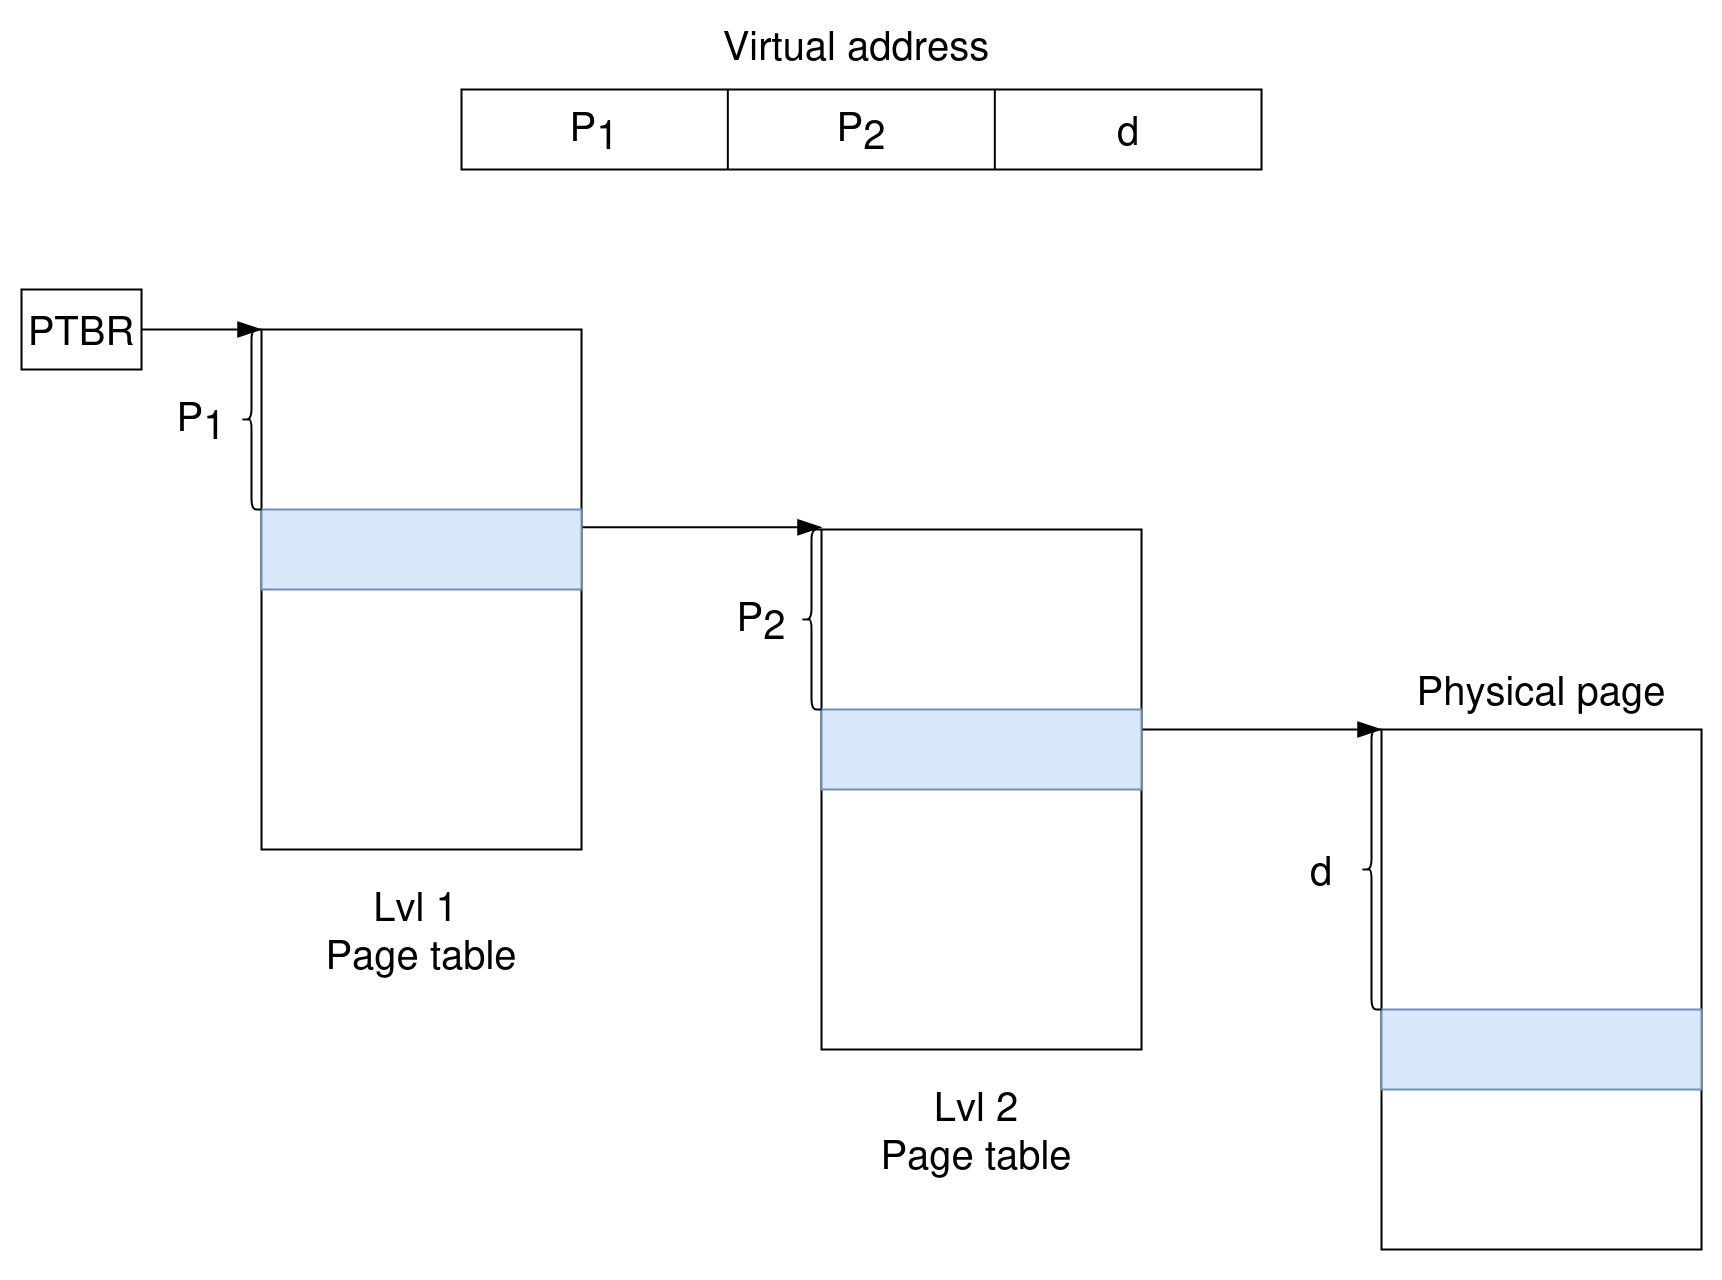
\includegraphics[width=0.7\textwidth]{hierachical-page-table.png}
  \caption{Hierarchical page table}
  \label{fig:hierarchical_page_table}
\end{figure}


\subsubsection{Inverted page table}

The inverted page tables take different approach.
Instead of defining page table for virtual address space, the table is constructed for physical memory.
The page table is in fact indexed using physical frame numbers.
The advantage over hierarchical page tables is that, the size of page table is related to the size of physical memory, and there is only one page table in the system.

Because page table is used to translate virtual addresses to physical ones, it would be hard to find page table entry knowing only virtual address.
To find proper PFN a hashing scheme is used on virtual page numbers.
Additionally, to avoid collisions, an structure called {\it hash anchor table} is used to store information about collision chains.

Inverted page tables are not common in practice, because usually it takes more memory accesses to read single PTE.

\begin{figure}[h]
  \centering
  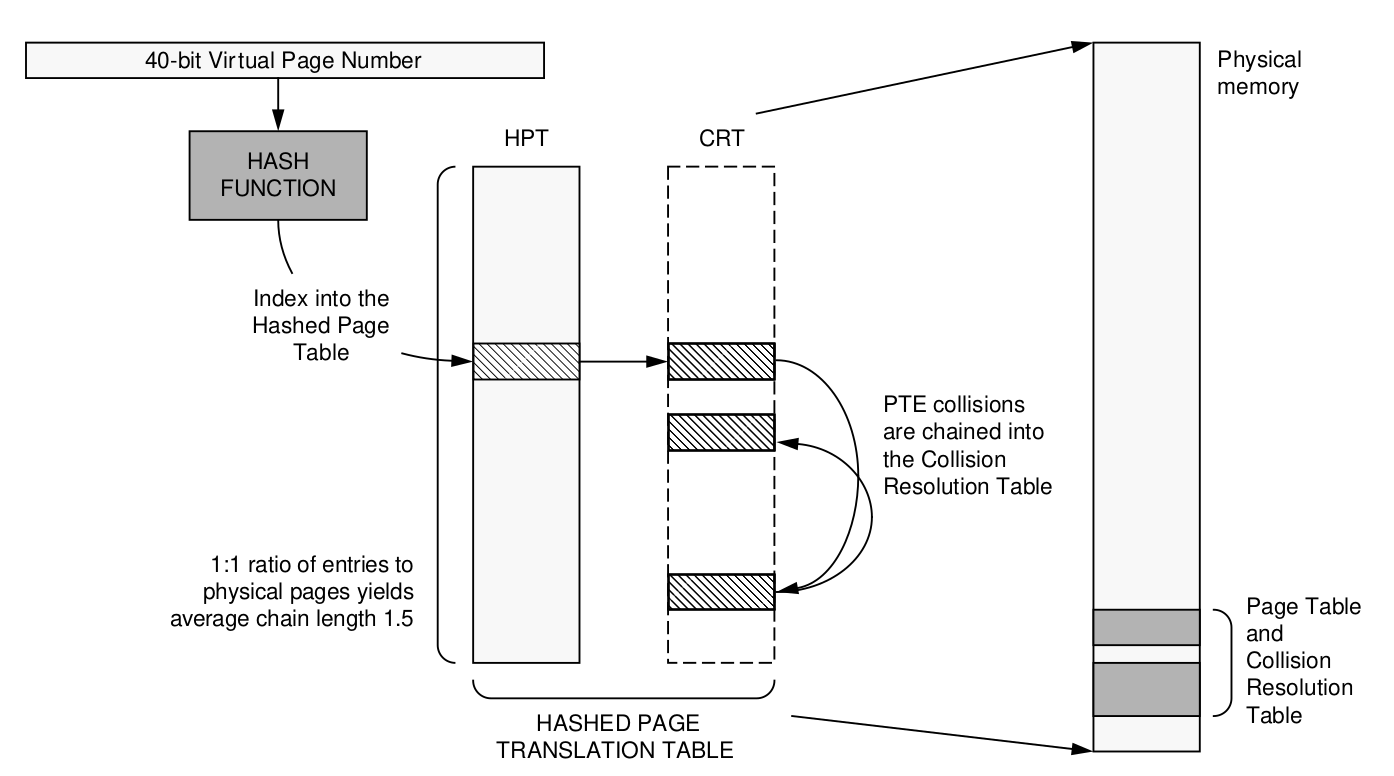
\includegraphics[width=0.9\textwidth]{memorysystems-inverted-page-table.png}
  \caption{Inverted page table \cite{memorysystems}}
  \label{fig:memorysystems:inverted_page_table}
\end{figure}

The details of page table designs, as well of real examples of their implementation can be found in \cite{memorysystems}.

\subsubsection{TLB}

The {\it translation look-aside buffer (TLB)} is a hardware designed to reduce the time it takes the MMU to read the PTEs.
It stores the most recently used page table entries because they are likely to be used again in a short time.
When making changes to the page table, kernel has to also ensure that the TLB is updated (usually by removing the modified PTEs from it).

TLB behaves like a cache for page table of current process, hence after a context switch all entries that was used by the previous process must be invalidated.
There are two ways of doing that: invalidating whole TLB after the context switch or identifying valid pages using ASID.

For more details on the design of TLB, see \cite{memorysystems}.

\subsection{Page fault}

As described in earlier sections, there are situations where memory access may fail
(either because memory is not available or because it has the wrong access permissions).
These situations must be handled by the kernel without bringing down the entire system.
When a bad memory access occurs, the {\it page fault} exception is thrown by the MMU.
The kernel must catch it, determine what caused the fault, and decide what action to take to recover from it.

We can classify page faults into 3 categories based on severity: minor and major page fault, and segmentation fault.
Minor page fault is when the page is in the main memory, but it is not referenced from page table.
In that case only page table of the process must be updated.
Major page fault happens, when page is in backing storage.
Then it has to be fetched into the main memory and proper mapping must be inserted into page table.
In the last case, the referenced page doesn't exist at all or process doesn't have a permission to perform requested memory access (e.g. write to read only page).

In fact, page faults may be triggered also by OS kernel.
Both major and minor page faults can be handled gracefully no matter in which context they happened.
The page used by kernel or user will be available after some time, because it exists.
When they happen, the page fault handler is invoked to inspect the VM~map of the process memory and determine if requested access was valid.
If that is true, the page must be made available.
By reading the VM~map of the process, it can be found where that page is stored.
There are three cases: page is actually in memory, page is in backing storage or page is not created yet.
If page does not exist it must be created or read from proper resource to be inserted into main memory.
To record information about new page or page fetched from backing storage, there must be allocated new frame in the memory and new mapping inserted into page table.

Segmentation fault cannot be handled, because it is triggered by an invalid memory access.
If it is triggered by the kernel it might cause kernel panic and bring down entire system.
When caused by the process, it isn't dangerous for the system because kernel can inform the process about it or terminate the process.
To convey the information about segmentation fault kernel sends \mintinline{c}{SIGSEGV} signal to the process.

\section{Kernel virtual memory}

In this thesis we focus on the virtual memory of user processes,
but a comment on how the kernel uses virtual memory may also be relevant.

The kernel also runs in virtual memory.
Right after it initializes all the structures needed to manage virtual memory, it switches to using virtual addresses.
This means that the kernel must also have a \mintinline{c}{pmap} structure to define the translations used by the MMU.

Even though the kernel uses virtual memory, it doesn't use all the features available to user processes.
Most of the memory pages used by the kernel are wired, and thus cannot be swapped out to make sure the kernel doesn't crash.

There are two main arguments for making kernel memory wired:
\begin{itemize}
  \item Some parts of the kernel need to be in memory at all times.
    The critical parts of the kernel may be impossible to fetch from backing storage.
    For example, if the code responsible for handling page faults is swapped out,
    it will be impossible to bring it back (because it is needed to fetch the pages from memory).
  \item There is also code that is executed very often and needs to be loaded quickly.
    If it were to be swapped out, it could cause a very long delay, which would be inconvenient for users.
\end{itemize}

Kernel memory is located at high addresses in the virtual address space.
It is always there, no matter what user process is running.
The part of pmap that describes the kernel address space is always there,
and doesn't change when process pmaps are swapped because the running process is changed.
Thanks to this, the kernel memory is always available to the kernel, no matter in which context the kernel is running.
It also allows the kernel to access the memory of the current process
(e.g. to copy some data to the buffers of the process as a result of a requested system call).

The kernel manages its memory in a different way than the processes.
It requires more sophisticated memory allocation mechanisms (e.g. slab allocators).
The details of kernel memory management are described in \cite{mckusick}, using the FreeBSD kernel as an example.

